% Déclaration du type de document (report, book, paper, etc...)
\documentclass[a4paper, 12pt]{paper} 
 
% Package pour avoir Latex en français
\usepackage[utf8]{inputenc}
\usepackage[T1]{fontenc}
 
% Quelques packages utiles
\usepackage{listings} % Pour afficher des listings de programmes
\usepackage{graphicx} % Pour afficher des figures
\usepackage{amsthm}   % Pour créer des théorèmes et des définitions
\usepackage{amsmath}
\usepackage{microtype} % Optical margins FTW
\usepackage{url}
\usepackage{booktabs} % Allows the use of \toprule, \midrule and \bottomrule in tables for horizontal lines
\usepackage[per-mode=symbol]{siunitx}
\usepackage{floatrow}
\usepackage{caption}
\usepackage{subcaption}
\usepackage{fullpage}
\usepackage{lipsum}



\author{Loïc Amez-Droz \and Florian Reinhard}
\title{Imaging}

% Début du document
\begin{document}
\begin{titlepage}
\begin{center}
    \textsc{\LARGE École Polytechnique Fédérale de~Lausanne}\\[1.5cm] 
    {\huge \bfseries Optical Engineering: Multimode Fibre}\\[0.4cm] 
    \begin{tabular}{|p{5cm}|p{4cm}|}
        \hline
        Group & C-XX \\ \hline
        Students & Loïc \textsc{Amez-Droz} \newline Florian \textsc{Reinhard} \\ \hline
        Date of lecture & 13.03.2015 \\ \hline
        Date of final report return & 20.03.2015 \\ \hline
    \end{tabular}
\end{center}


\begin{abstract}
    \lipsum[3]
\end{abstract}
 
\vfill
\end{titlepage}

\section{Procedures and results}
\subsection{Zero optical path difference}

\begin{figure}[H]
    \begin{subfigure}[t]{0.45\textwidth}
        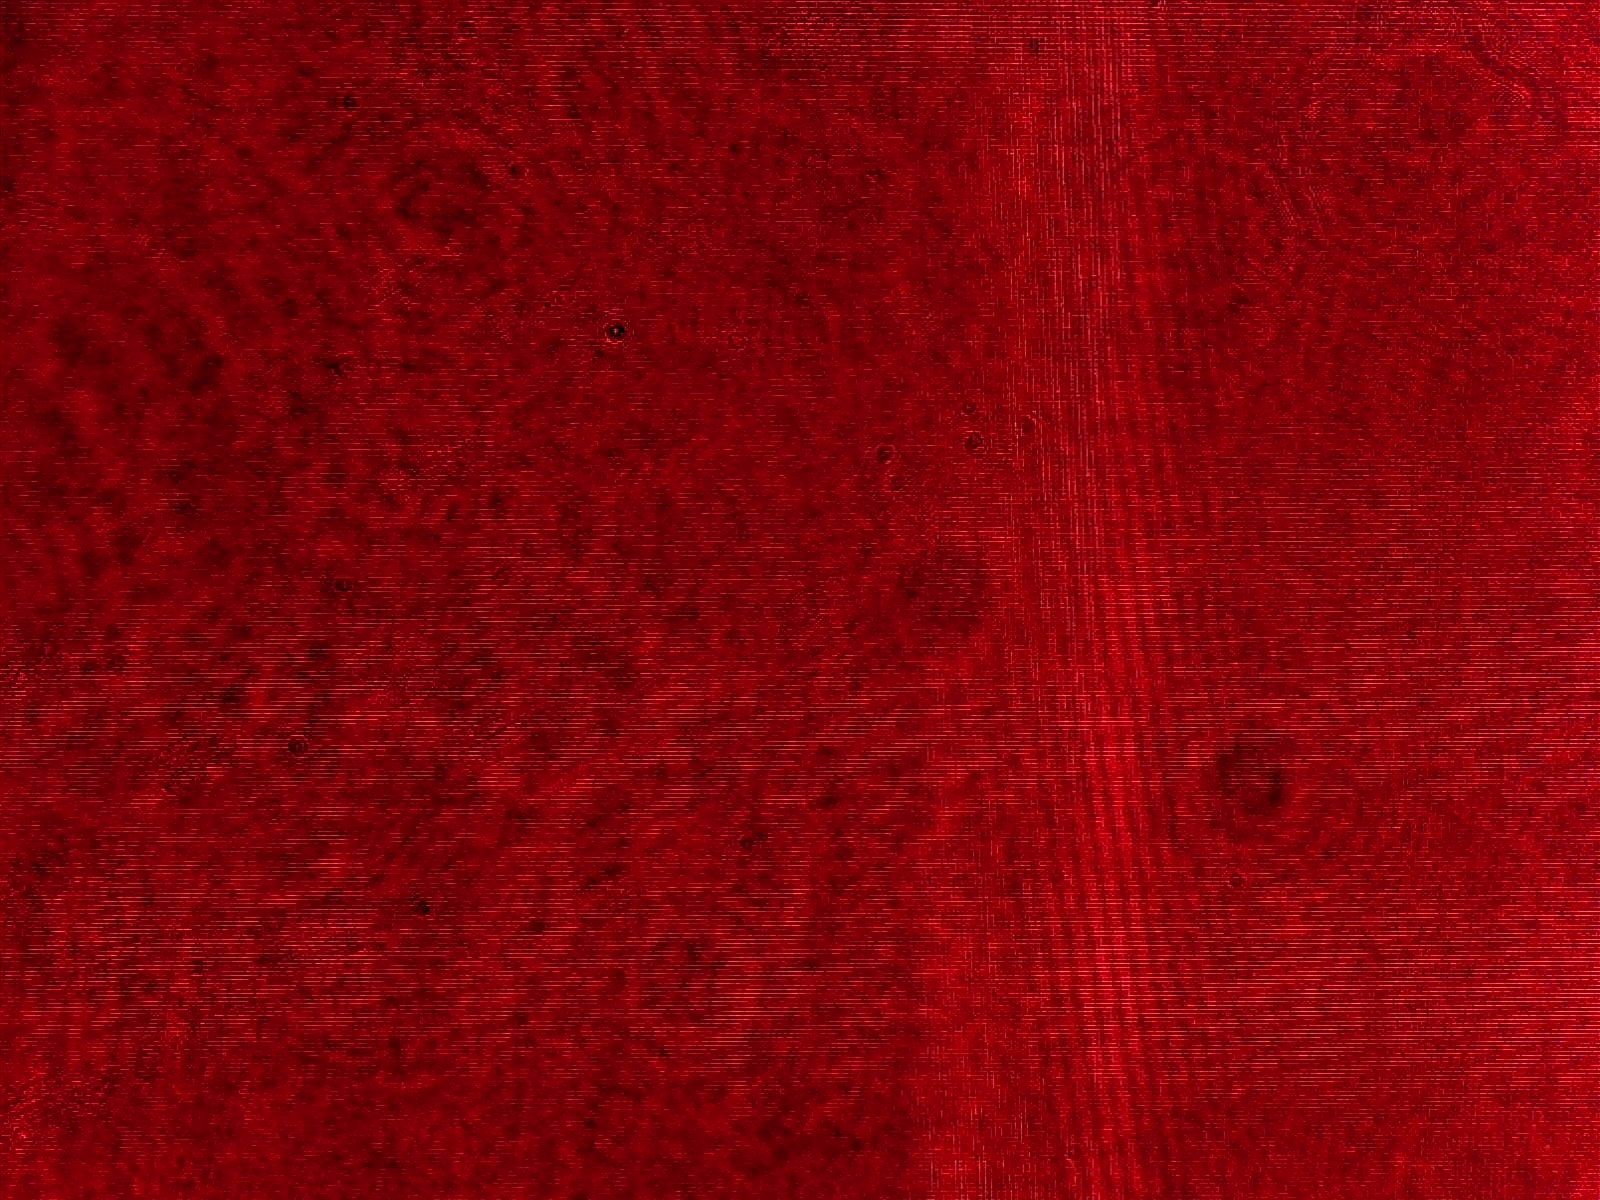
\includegraphics[width=\textwidth]{img/ZOPD_high}
        \caption{High intensity.}
    \end{subfigure}
    \begin{subfigure}[t]{0.45\textwidth}
        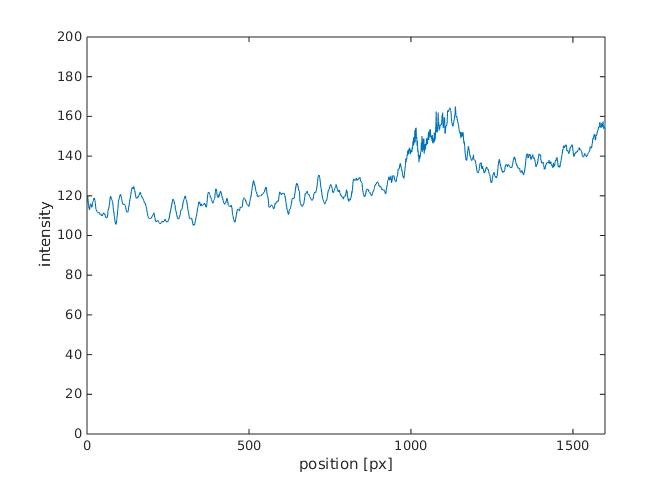
\includegraphics[width=\textwidth]{img/ZOPD_high_line}
        \caption{High intensity line graph.}
    \end{subfigure}
    \begin{subfigure}[t]{0.45\textwidth}
        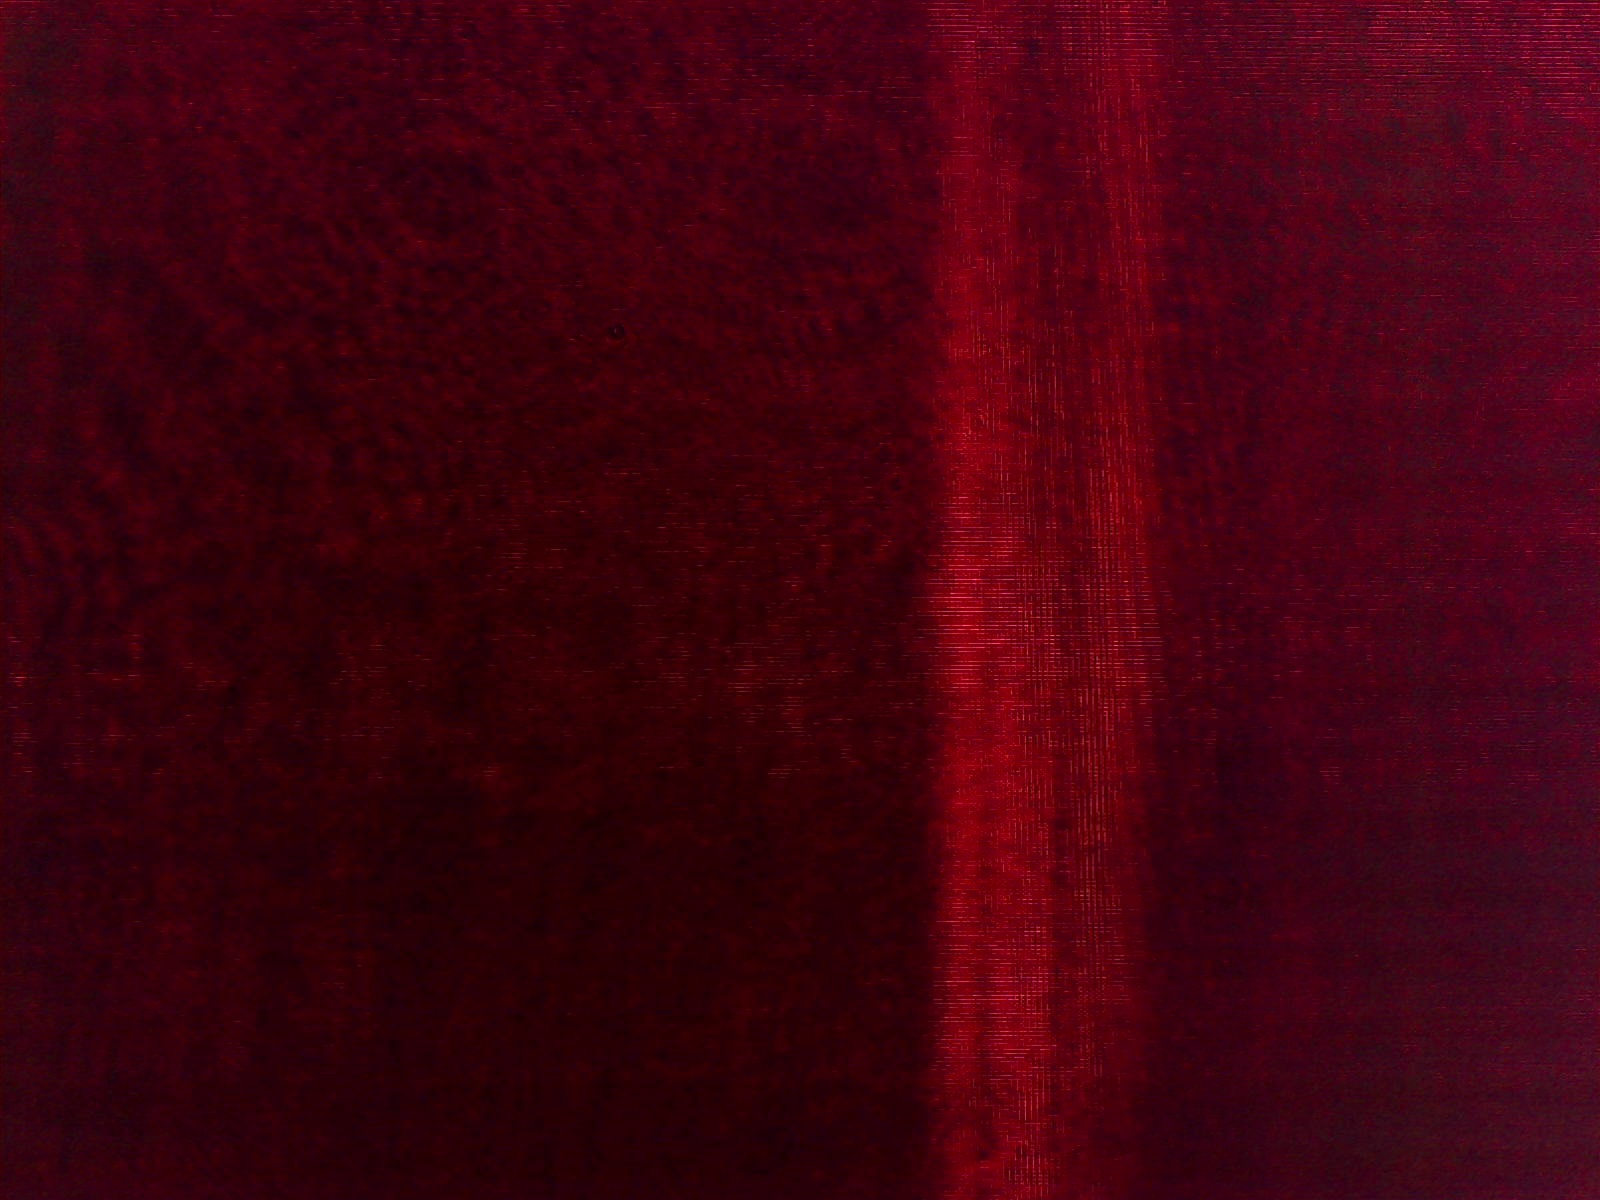
\includegraphics[width=\textwidth]{img/ZOPD_low}
        \caption{Low intensity.}
    \end{subfigure}
    \begin{subfigure}[t]{0.45\textwidth}
        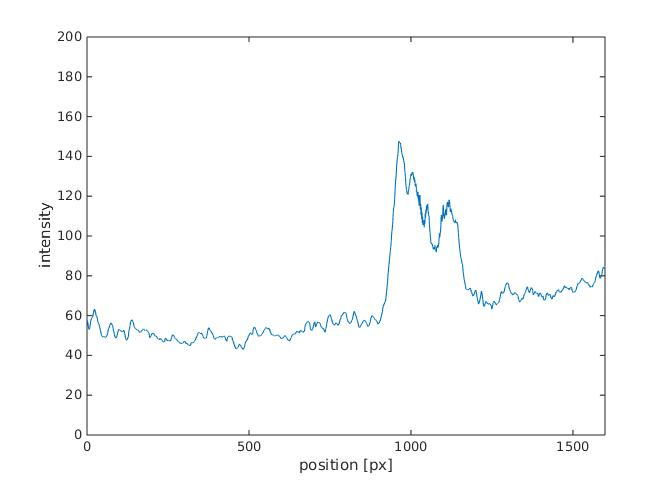
\includegraphics[width=\textwidth]{img/ZOPD_low_line}
        \caption{Low intensity line graph.}
    \end{subfigure}
    \caption{Zero optical path difference. The intensity is a result of either positive or negative interfence and can be manipulated by pressing slightly on base plate of the system. The contrast is $C = 0.39$.}
\label{fig:zopd}
\end{figure}

\subsection{Measurement of laser fringe contrast}

\begin{figure}[H]
    \begin{subfigure}[t]{0.40\textwidth}
        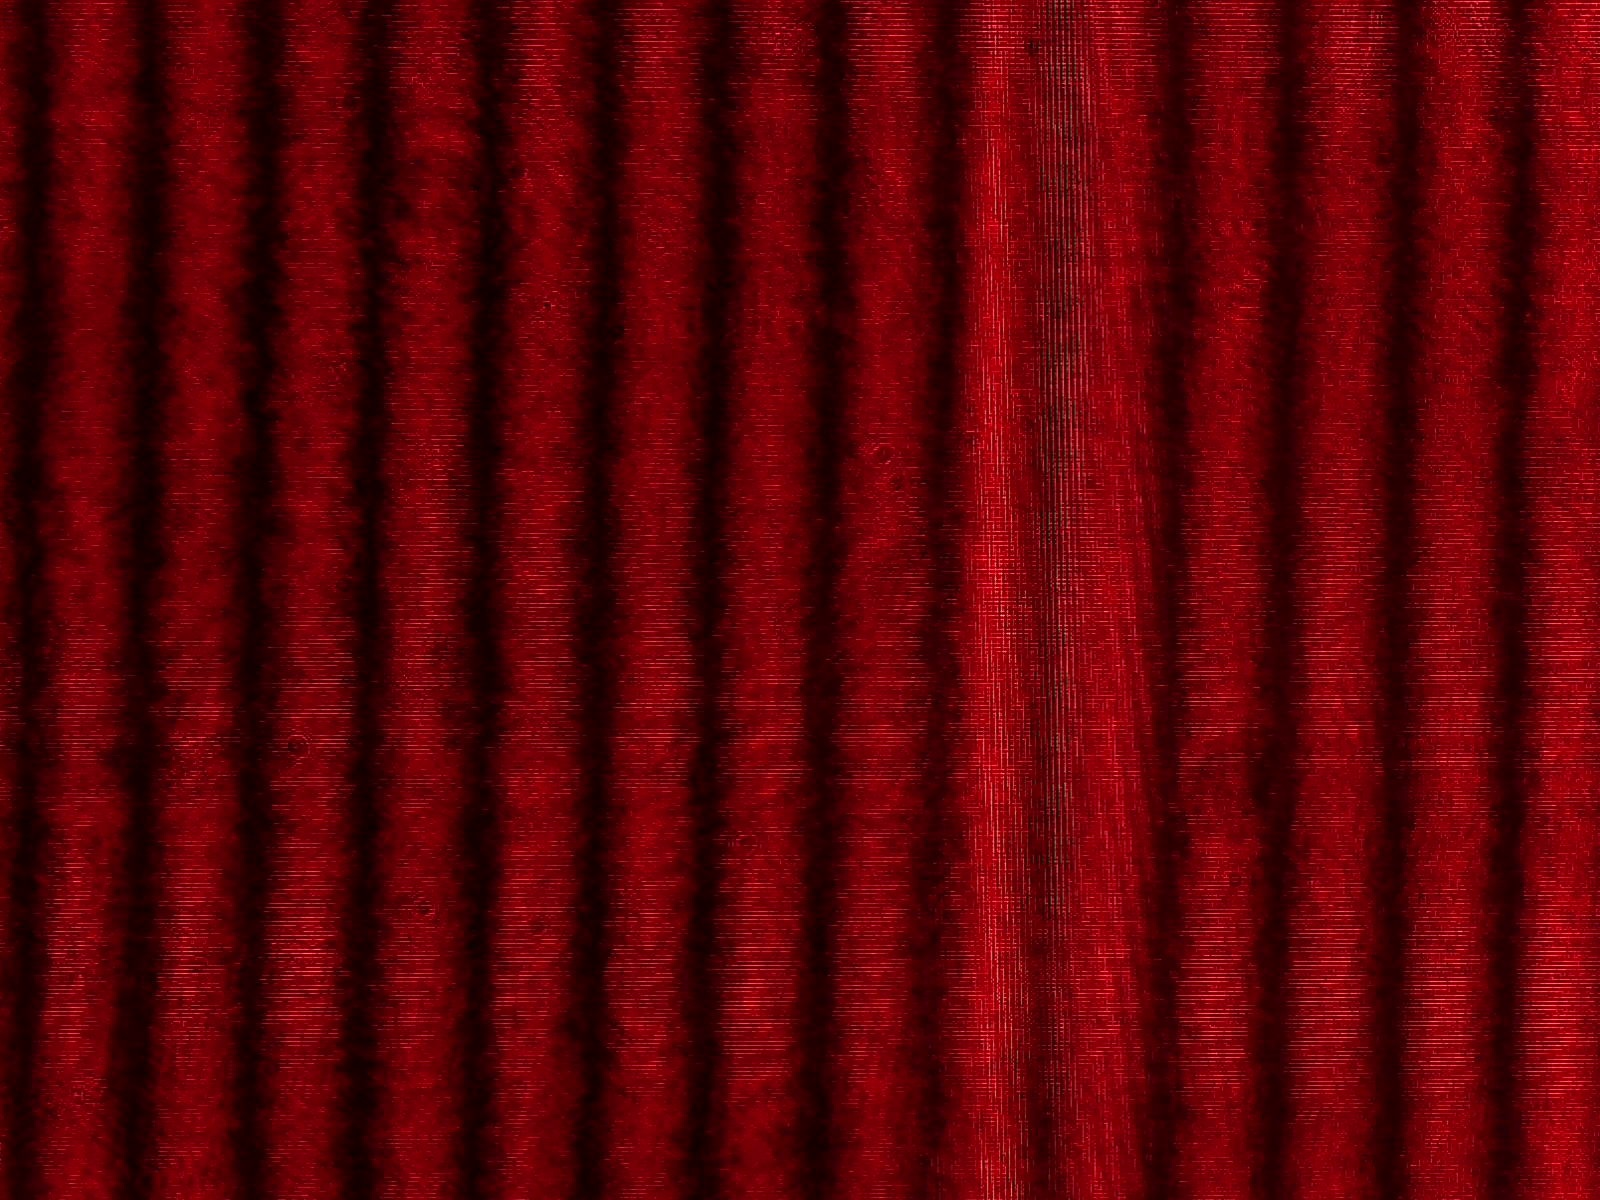
\includegraphics[width=\textwidth]{img/107}
        \caption{High contrast.}
    \end{subfigure}
    \begin{subfigure}[t]{0.45\textwidth}
        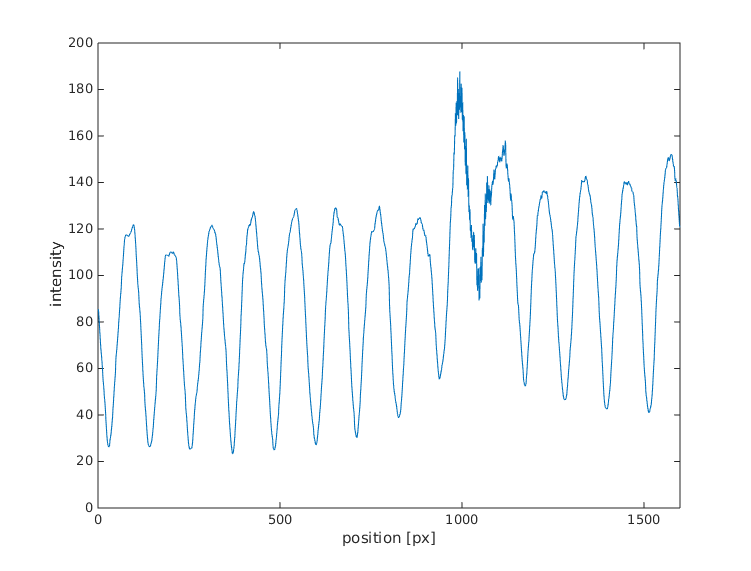
\includegraphics[width=\textwidth]{img/high_contrast_line}
        \caption{High contrast line plot.}
    \end{subfigure}
    \begin{subfigure}[t]{0.40\textwidth}
        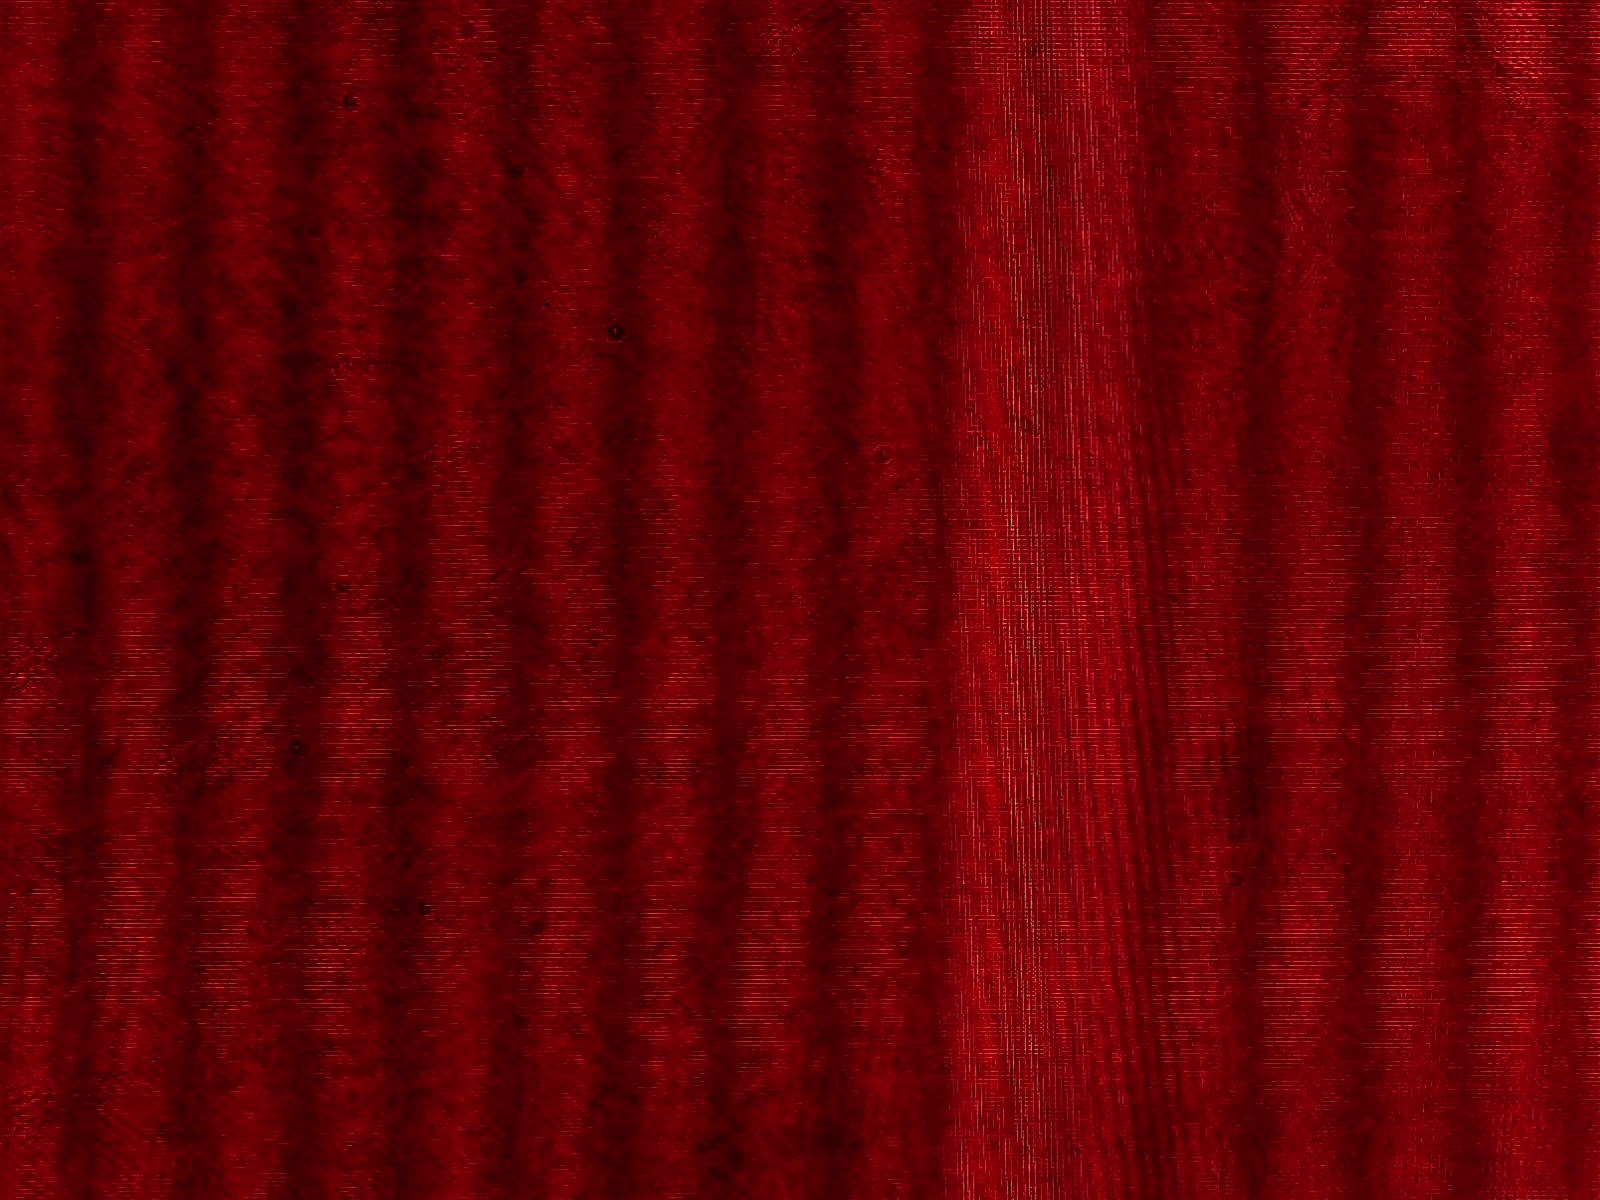
\includegraphics[width=\textwidth]{img/137}
        \caption{Medium contrast.}
    \end{subfigure}
    \begin{subfigure}[t]{0.45\textwidth}
        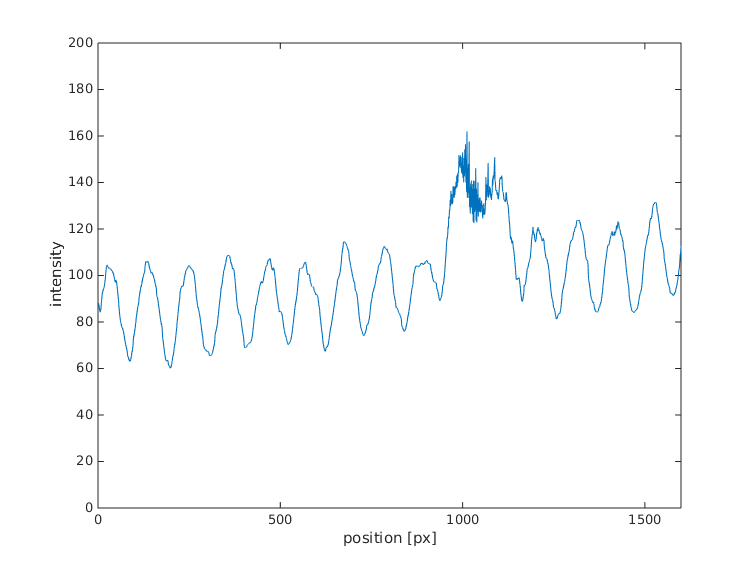
\includegraphics[width=\textwidth]{img/medium_contrast_line}
        \caption{Medium contrast line plot.}
    \end{subfigure}
    \begin{subfigure}[t]{0.40\textwidth}
        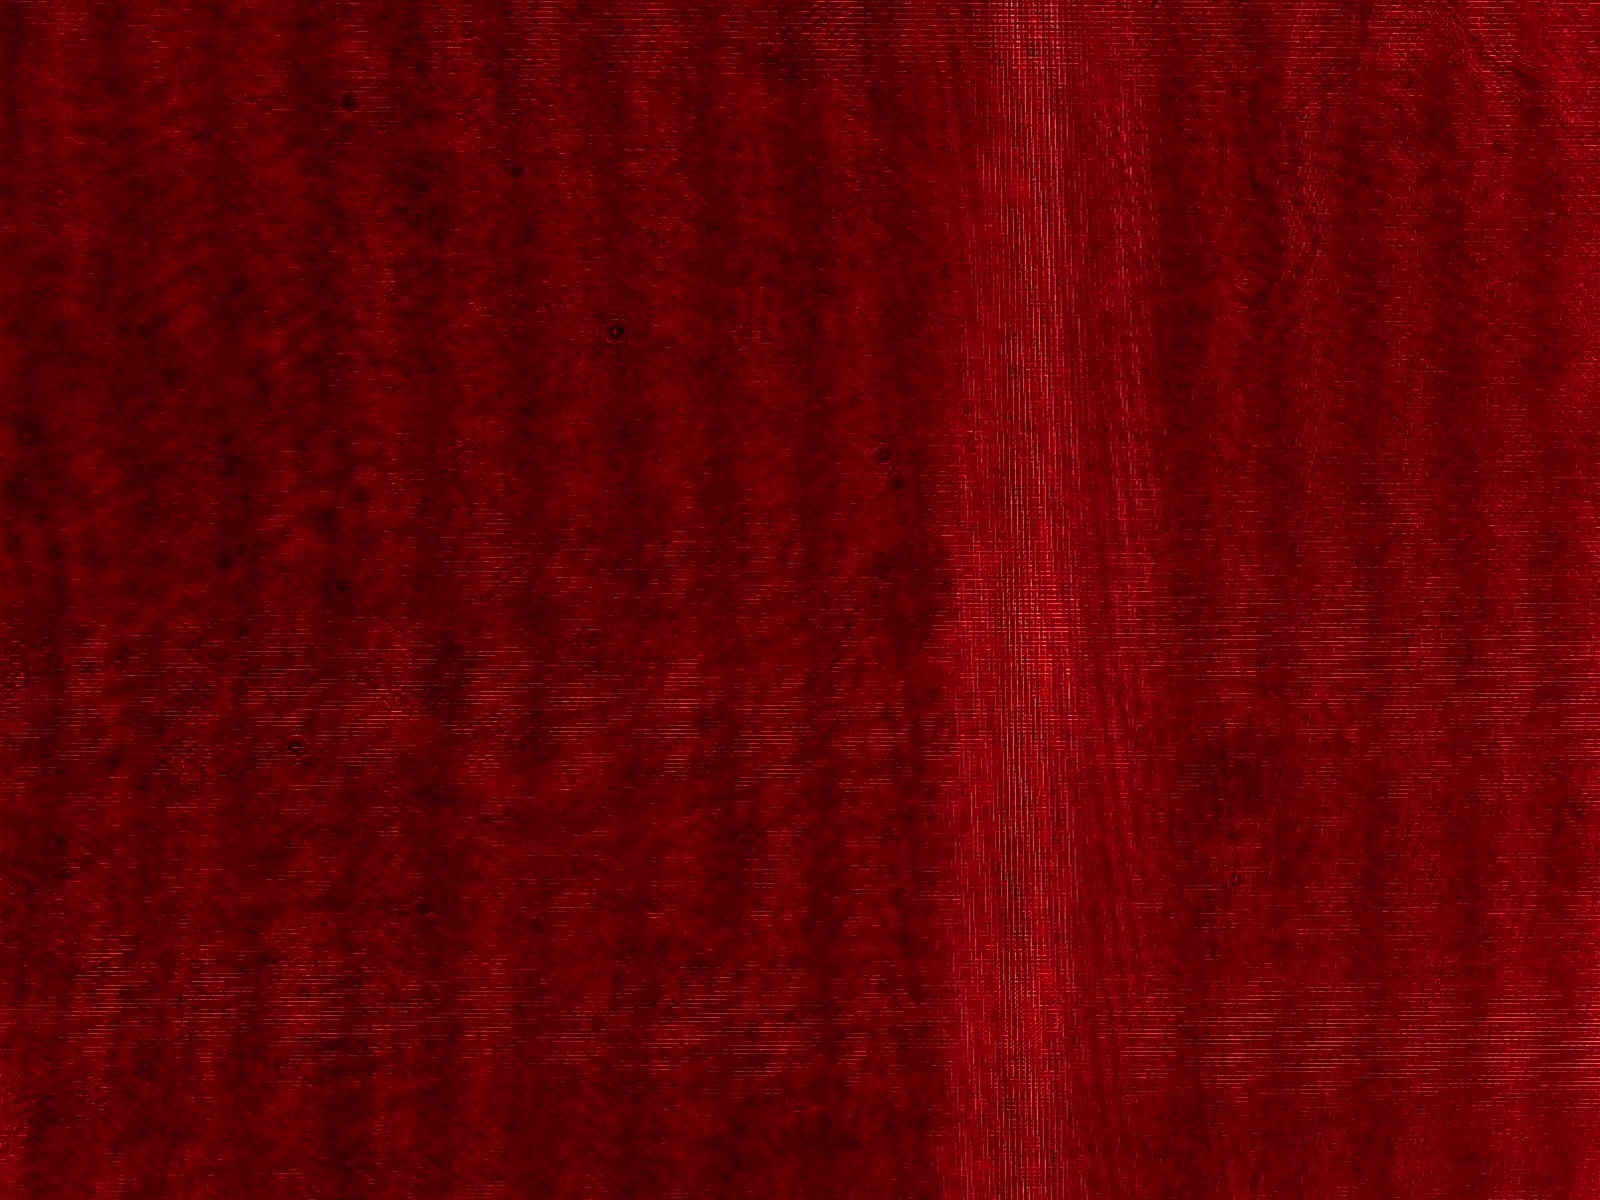
\includegraphics[width=\textwidth]{img/197}
        \caption{Low contrast.}
    \end{subfigure}
    \begin{subfigure}[t]{0.45\textwidth}
        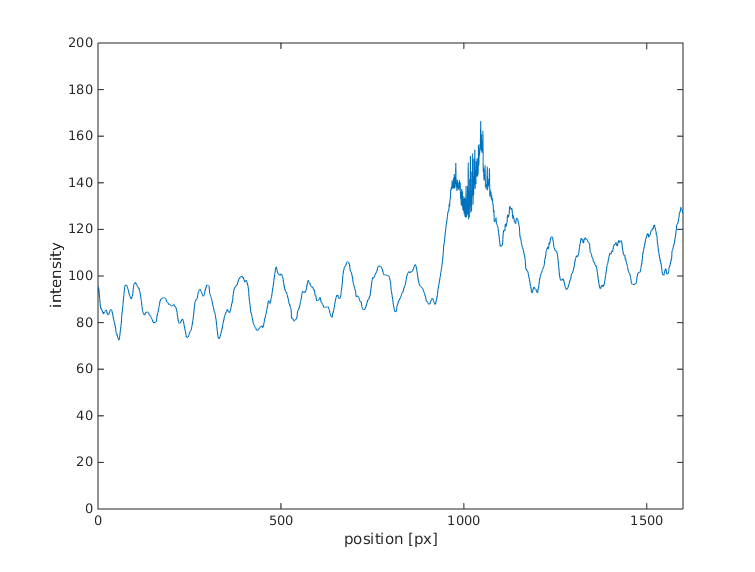
\includegraphics[width=\textwidth]{img/low_contrast_line}
        \caption{Low contrast line plot.}
    \end{subfigure}
    \caption{Fringes with different contrasts and their corresponding line plots. Tha change of contrast is due to a change of the optical path difference.}
\label{fig:contrast}
\end{figure}

\begin{figure}[H]
    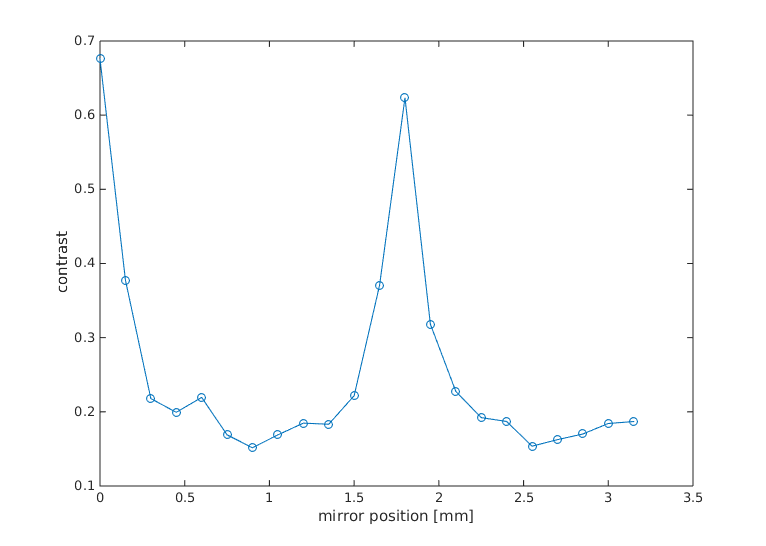
\includegraphics[width=0.6\textwidth]{img/contrast_graph}
    \caption{The contrast as a function of the measurement position. We deduce $\Delta z = \SI{1.8}{\milli\meter}$ as the period of the variation.}
\label{fig:contrast_graph}
\end{figure}

With the period of the variation $\Delta z$ deduced in figure~\ref{fig:contrast_graph}, we can calculate the spectral width $\Delta \lambda$ (equation~\ref{equ:beating_distance}).

\begin{equation}
    \Delta \lambda = \frac{\lambda^2}{\Delta z} = \frac{{\left( \SI{635}{\nano\meter} \right)}^2}{\SI{1.8}{\milli\meter}} = \SI{0.22}{\nano\meter}
    \label{equ:beating_distance}
\end{equation}

\subsection{Phase shifting interferometry}

Performing finger pressure on the support, we search to observe \SI{180}{\degree} phase shifting.

\begin{figure}[H]
    \centering
    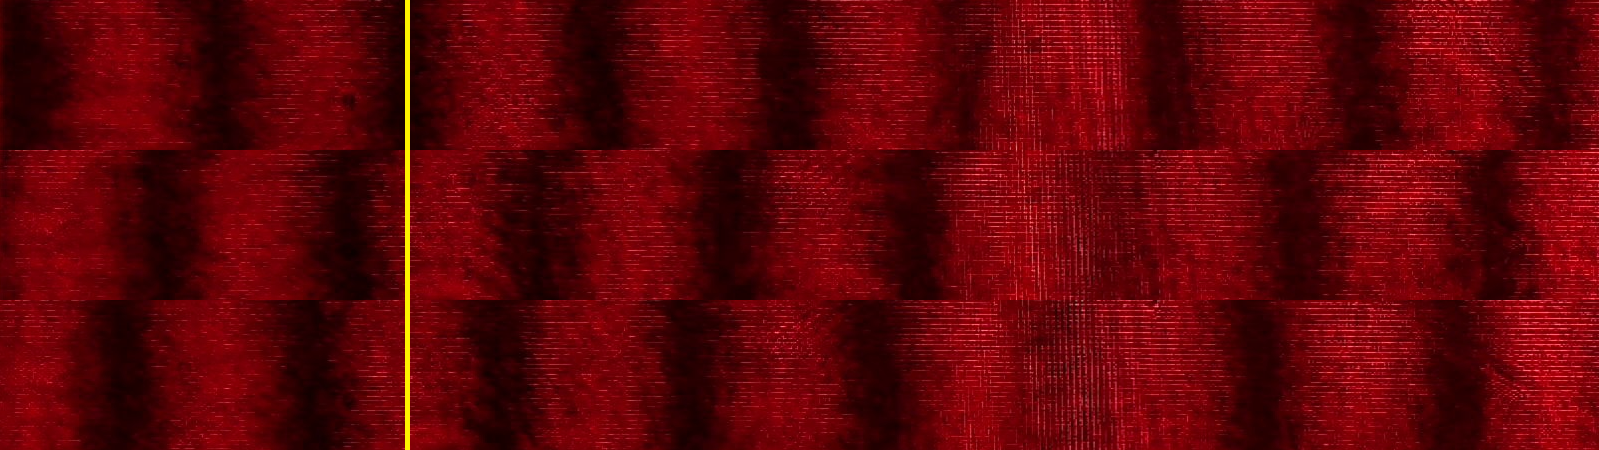
\includegraphics[width=1.0\textwidth]{img/phase_fringes}
    \caption{Different phase shifts.}
\label{fig:phase_fringes}
\end{figure}

\begin{figure}[H]
    \begin{subfigure}[t]{0.45\textwidth}
        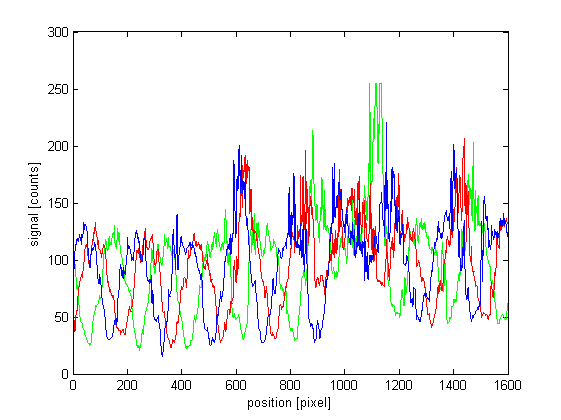
\includegraphics[width=\textwidth]{img/intensity_1_line}
        \caption{Intensity of the center line of three different phases.}
    \end{subfigure}
    \begin{subfigure}[t]{0.45\textwidth}
        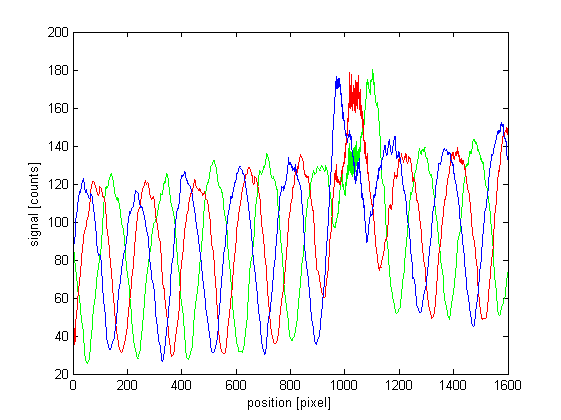
\includegraphics[width=\textwidth]{img/intensity_200_lines}
        \caption{Intensity averaged over 200 lines.}
    \end{subfigure}
    \begin{subfigure}[t]{0.45\textwidth}
        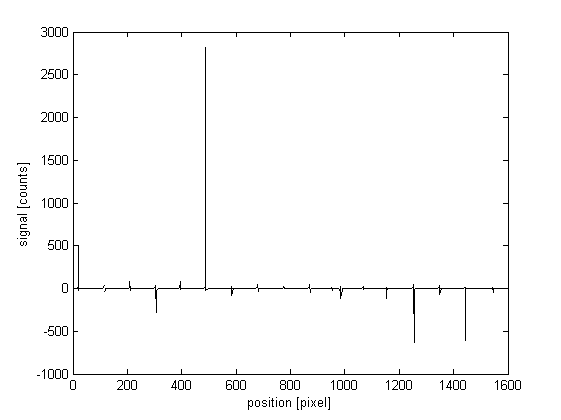
\includegraphics[width=\textwidth]{img/tangent}
        \caption{Tangent plot.}
    \end{subfigure}
    \begin{subfigure}[t]{0.45\textwidth}
        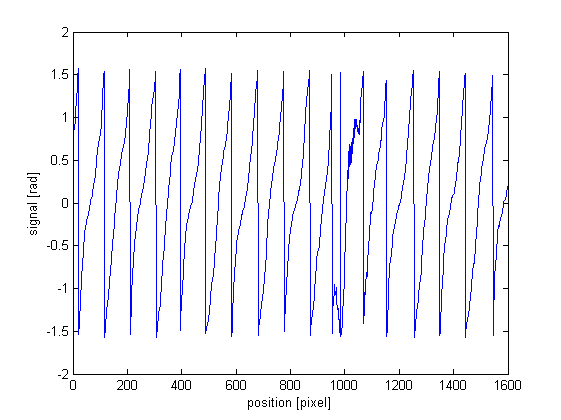
\includegraphics[width=\textwidth]{img/phase}
        \caption{Phase between $-\frac{\pi}{2}$ and $\frac{\pi}{2}$.}
    \end{subfigure}
    \begin{subfigure}[t]{0.45\textwidth}
        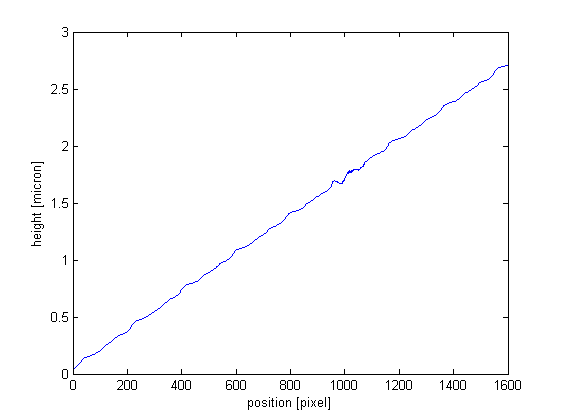
\includegraphics[width=\textwidth]{img/phase_developped}
        \caption{Height difference as a funciton of the position (unwinded phase).}
    \end{subfigure}
\label{fig:phase_shift}
\end{figure}

We can observe phase shifting spotting destructive and constructive interferences.
Observing the destructive and constructive fringes we feel there haven’t the same width.
It’s wrong, there are exactly identical.
The error can result by overexposure or eyes sensibility or brain color treatment.
Significant irregularities on the intensity diagrams result by a blurred column appearing on all our pictures.
On the last picture we determinate the slope $\left( \SI{1.65e-3}{} \right)$.
So the angle which generate a \SI{180}{\degree} shift is $\alpha = \SI{0.06e-3}{\degree}$.
This angle represent a \SI{635/2}{\nano\meter} distance variation ($\frac{1}{2}$ coefficient because the ray cover the distance at back and forth).
These values correspond to the interferometer resolution. 

\subsection{Web-Example}

\begin{figure}[H]
    \begin{subfigure}[t]{0.5\textwidth}
        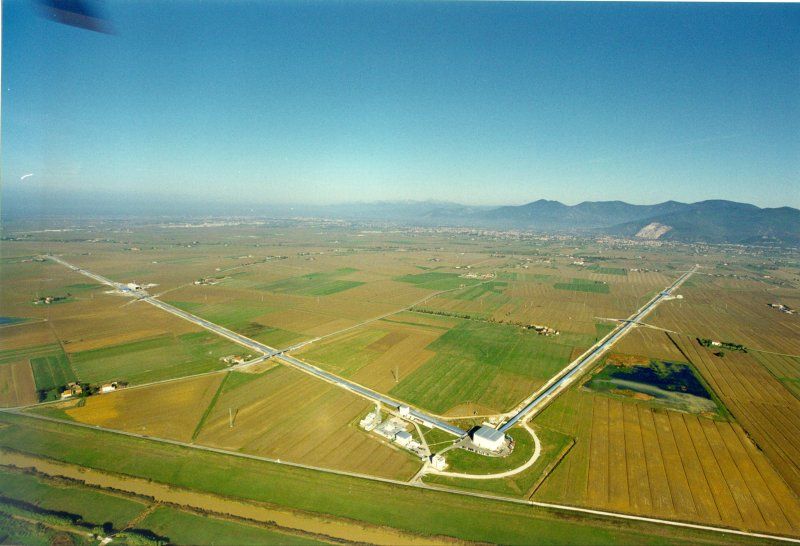
\includegraphics[width=\textwidth]{img/virgoview}
    \end{subfigure}
    \begin{subfigure}[t]{0.4\textwidth}
        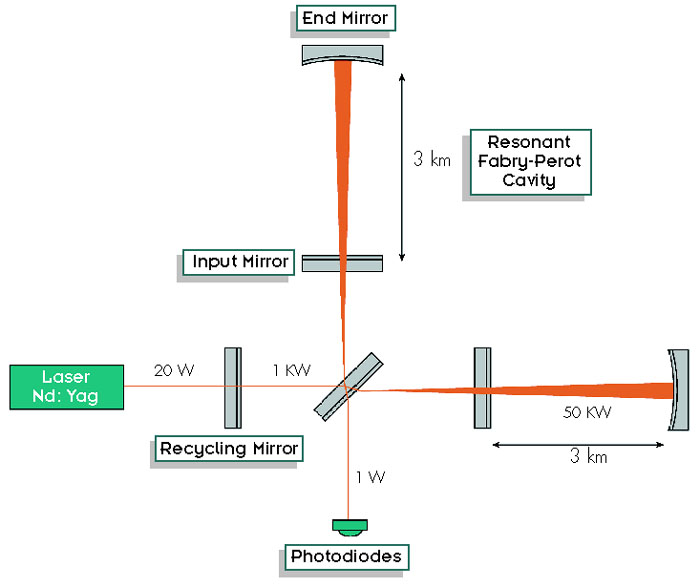
\includegraphics[width=\textwidth]{img/schema3.jpg}
    \end{subfigure}
    \caption{Sources: Laboratoire d’Annecy-le-Vieux de Physique des Particules and EGO (European Gravitational Observatory)}
\label{fig:web_example}
\end{figure}

The Virgo is a gravitational wave detector built in Italy in the site of EGO.
It’s a Michelson laser interferometer which has two arms \SI{3}{\kilo\meter} length.
The effective optical length of each arm is extended by the mirrors up to 100 kilometers.
His frequency range sensibility extends from \SI{10}{\hertz} to \SI{10}{\kilo\hertz}.
This range should allow detection of gravitational radiation produced by supernovae and the coalescence of systems in the Milky Way and in outer galaxies.

\section{Discussion}

It was interesting to experiment with a interferometer and to see the incredibly small distances and angles that can be resolved using this technology, as well as the difficulties that come along with setting up such a system.

\end{document}
